\chapter{Анализ масштабируемости, параллельной эффективности и ускорения параллельной ВС}
			%	ОБЩЕЕ ПРАВИЛО ДЛЯ ВТОРОЙ ГЛАВЫ: НЕ ПЛАНРИРОВАТЬ ЧТО_ТО НОВОЕ И ОЧЕНЬ ХОРОШЕЕ ЧЕГТО НЕТ, А ПОДКРЕЛЯТЬ И УИСИЛВАТЬ ТО, ЧТО РЕАЛЬНО ЕСТЬ.
			%	ЕСЛИ У НАС СЛАСБОСТЬ В ОБЛАСТИ АНАЛИЗА КОММ СТРУКТУРЫ - НУ И ЛАДНО, И ПУСТЬ ОНА БУДЕТ. ГОВОРИТЬ БОЛЬШЕ О МАСШТАБИРУЕМОСТИ. А КОРММ СТРУКТУРУ АНАЛИЗИРПОВАТЬ ЧЕРЕЗ ПЕРЕСЫЛКИ ЧАСТИЦ
			%	НАША ИДЕЯ не ПОДМЕНЯТЬ СОБОЙ ДИАГНОСТИКУ АРХИТЕКТУРЫ, а мерять И ОПРЕДЕЛЯТЬ ВСЕ ЧЕРЕЗ ИЗМЕРЕНИЯ ВРЕМЕН ПО PIC
				В четвертой главе предложена методика интегральной оценки тестируемой ВС с помощью измерения масштабируемости с расчетах по методу частиц в ячейках и определения на основе измерений возрастания потока данных в коммуникационной сети ВС.
%				На основе данных о пересылке модельных частиц измерена производительность коммуникационной сети ВС, при этом важно отметить преимущества использованного метода измерений: пересылка данных имеет высокую степень нерегулярности, а также большой объем, что означает проведение тестирования на большой нагрузке, и возможность широкого применения полученных таким образом данных.
%				Также предложена и апробирована методика определения фактически соседних (с точки зрения MPI) узлов ВС.  
							
			\section{Определение понятий эффективности, масштабируемости и ускорения}
			%\textbf{Степаненко, книжка"высокопроизводительные вычисления", учебник Воеводина}
			
			Выписано определение эффективности параллельной реализации программ, сильной и слабой масштабируемости, ускорения при распараллеливании.
			
			В частности, ускорение параллельного алгоритма для $N$ процессоров, определяется как:
			$$
			S_N = \frac{T_1(n)}{T_N(n)}
			$$  
			здесь $T_1$ - время исполнения алгоритма на одном процессоре, $T_N$ - на $N$ процессорах, величина $n$ характеризует вычислительную сложность решаемой задачи, для определения ускорения существенно, что задачи, решаемые на 1 и на $N$ процессорах имеют одинаковую сложность.
			Далее, эффективность распараллеливания вычисляется как
			$$
			\eta_N = \frac{1}{N}\frac{T_1(n)}{T_N(n)}
			$$  
			эта величина иногда называется эффективностью в сильном смысле (англ. strong efficiency). Кроме того, часто используется эффективность в слабом смысле (англ. weak efficiency):
			\begin{equation}
			\label{weak_eff}
			\eta^{weak}_N = \frac{T_1(1)}{T_N(N)}
			\end{equation}
			здесь, в отличие от определения ускорения, задачи, решаемые на одном и на $N$ процессорах, имеют различную сложность, т.е. при увеличении количества процессоров в $N$ раз сложность задачи такжэе увеличивается в $N$ раз, и таким образом определяемая эффективность будет 100 \% в том случае, если время вычислений не возрастает при увеличении сложности задачи пропорциональном увеличению количества процессоров.   
			
			Приведены различные используемые варианты этих определений, перечислены факторы, влияющие на  значения этих величин для конкретной ВС, а именно скорость обмена данными и структура коммуникационной сети ВВС, алгоритмы реализации MPI-процедур, в особенности коллективных, настройки коммуникационной системы (таймауты, размер системных буферов, и др.).
			%\textbf{написать формулы} 
			%\textbf{привести формулы из статьи в СибЖВМ}
			Для последующего анализа измереннного времени работы метода частиц в ячейках на параллельной ВС, и для прояснения зависимости этого времени от параметров расчета можно привести следующую схематическую формулу для длительности одного временного шага, аналогично статье (Вшивков В.А. и др., СибЖВМ, 2003):
			
			\begin{equation}
			\label{PIC-timestep}
			T=T_{F} \left ( \frac{N_x N_y N_z }{P_E}\right )+ T_{F,S}\left (N_y N_z\right ) + T_P\left(\frac{N_p}{P_E\times P_L}\right) +T_{P,S}\left (\frac{N_p*T_p}{P_E\times P_L}\right)
		\end{equation}
			 
		здесь $T_{F}$ - время вычисления электромагнитного поля, $N_x, N_y, N_z$ - размер расчетной сетки соответственно, по координатам $X$ $Y$ и $Z$, $P_E$ - количество процессоров для эйлеровой декомпозиции, т.е. для разделения расчетной области на подобласти, $T_{F,S}$ - время, затрачиваемое на персылку граничных значений полей и токов между подобластями, которое зависит только от $N_y$ и $N_z$ в силу того что на данный момент используется одномерная декомпозиция,  $T_P$ - время расчета движения частиц, $P_L$ - количество процессов (или потоков) для лагранжевой декомпозиции, т.е. для дополнительного разделения частиц подобласти на группы, вычисляемые на отдельных ядрах.
		
		

		
		
		\section{Анализ масштабируемости как интегральной характеристики ВС.}
		
		Во втором разделе приведены фактически измеренные на различных высокопроизводительных ВС графики масштабируемости и параллельной эффективности и на основе этих данных проведен анлиз коммуникационной сети данных ВС, в частности, для МВС-100К, рис. \ref{eff2}. 
		
		\begin{figure}[h]
			\begin{center}
				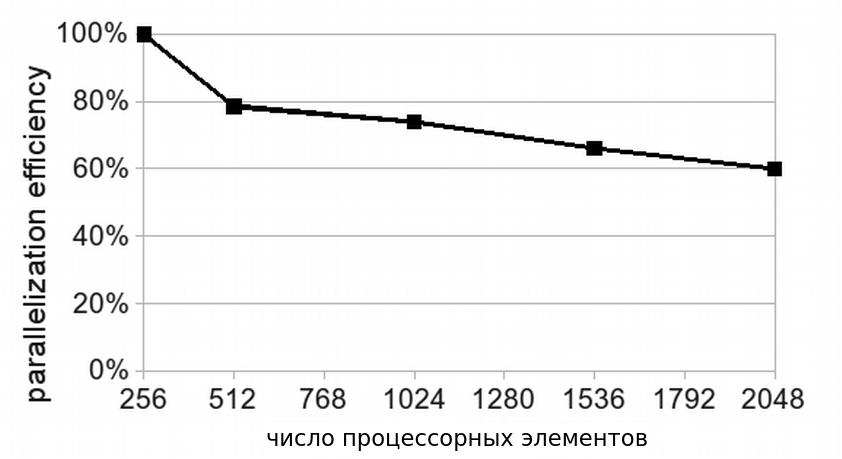
\includegraphics[height=5cm,keepaspectratio]{images/eff_weak_JSCC.png}
				\caption{
					Эффективность распараллеливания в слабом смысле, для МВС-100К, МСЦ РАН.
				}
				\label{eff2}
			\end{center} 
		\end{figure}
		
		Возможность проведения анализа коммуникационной сети с помщью расчетов по методу частиц в ячейках основана на известной информации о количестве пересылаемых данных и о виртуальной топологии, используемой в программе.
		
		Размер данных, перемещаемых между двумя соседними MPI-процессами равен $144 \times N_y N_z  $ байт. При этом в идеальном случае, когда соседние MPI-процессы находятся на соседних узлах, коммуникации происходят только между соседними узлами, и поток данных в системе в целом не возрастает с ростом количества используемых в расчете узлов.
		
		В частности, в расчете показанном на рис. \ref{eff2} использована эйлерова декомпозиция. Это означает, что используются только парные пересылки MPI, коллективные пересылки не используются, и поток данных через коммуникационную систему ВС в целом возрастать не должен. Если, тем не менее, он возрастает, что видно на рис. \ref{eff2} в виде снижения эффективности распараллеливания, то это может (при отсутствии коллективных операций), означать, что соседние с точки зрения MPI процессы находятся на физически удаленных друг от друга узлах параллельной ВС.
		
		Обозначая $k_{||}$ зависимость коэффициента при времени пересылок граничных условий от количества процессоров в формуле \ref{PIC-timestep}, так что 
		\begin{equation}
		T_{F,S} = k_{||} (P_E) \frac{N_y N_z}{P_E}
		\end{equation} 
		и подставляя формулу \ref{PIC-timestep} d \ref{weak_eff}, рассматривая только лишь время расчета и пересылок электромагнитного поля, можно получить 
		\begin{equation}
		k_{||} (P_E) = \frac{1}{\eta^{weak}(P_E)} - 1
		\end{equation}	  
		Таким образом величина $k_{||} (P_E)$  - \textbf{степень нелинейности} коммуникационной структуры параллельной ВС. Фактически она представляет собой отклонение от линейной функции для зависимости времени пересылок от количества процессоров. Он показывает предел возрастания потока данных через коммуникационную структуру ВС при увеличении количества процессоров, используемых в расчете. Эта величина характеризует, в какой степени при передаче информации между соседними процессами в MPI используются узлы параллельной ВС, не являющиеся ближайшими соседями. В силу того, что на значение эффективности оказывает влияние не только свойства оборудования, но и особенност реализации MPI, возникает необходимость разделить эти факторы. Это достигается с помощью привязки процессорв к узлам. 
		
		В итоге, такимобразом определенная  величина $k_{||} $ может быть использована как характеристика параллельной ВС, показывающая реально достижимую с помощью данной ВС эффективность и масштабируемость   
		
		\subsection{Измерение продолжительности параллельных коммуникаций и анализ характеристик и топологии коммуникационного оборудования}
		Здесь описано решение задачи об определении соседства процессов по реальным узлам. Это исключительно важно для производительности реальных задач, чтобы виртуально близкие (т.е. по номеру MPI-процесса) процессы исполнялись бы на соседних узлах многопроцессорной ВС. Для этого проводится обмен сообщениями между узлами, выделенными 
		для исполнения программы по топологии полного графа, и проводится анализ времени прохождения сообщений, рис. \ref{poly_all2all}.  
		
		Следует отметить, что такого этапа, с обменом сообщениями между всеми процессами в рамках метода частиц нет, поэтому, такой анализ проводится предварительно, перед запуском основной части программы.

		
		\begin{figure}[htb]
			\begin{center}
				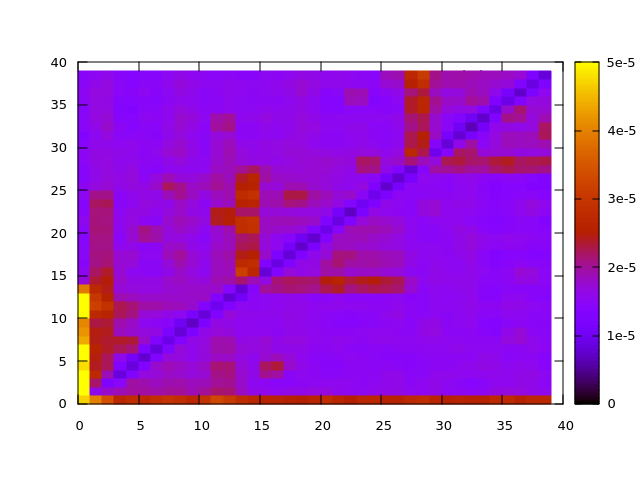
\includegraphics[height=7cm,keepaspectratio]{images/polytech_all_to_all.png}
			\end{center}
			\caption{Время пересылок для 40 MPI-процессов, расположенных на 10 узлах по 4 процесса, кластер «Политехник», СПбПУ. По осям X и Y отложены номера процессов, цветовая шкала показывает время пересылок в секундах.}
			\label{poly_all2all}
		\end{figure} 
		Узлы с минимальным временем считаются близкими, т.е. выясняется фактическая топология ВС. Это сопоставляется с известной информацией о размещении процессов по узлам.	Для повышения производительности приложения в дальнейшем целесообразно передвинуть соседние процессы на те узлы, где по факту меньше задержка по коммуникациям.
		
		%	\textbf{картинку из стьатьи все-со-всеми, (с Политеха)}. 
		%	1.измерение всех видов MPI-коммуникаций, сравнение одного с другим (Send, Isend, Bsend) - и увязатиь это с алгоритмом
		%	2. варьирование размера сообщений и пр. параметров
		
	%	\textbf{материал статьи НГУ ИТ  с более аакуратным анализом}
        \section{Оценки параллельной масштабируемости на основе измерений времени прохождения сообщений}
        
        С этим связан основные вопросы настоящей статьи: 
        что, если группа процессов, которые должны осуществлять коллективные пересылки, окажется размещенной на узлах суперЭВМ, расположенных физически далеко друг от друга, так что время выполнения этих пересылок будет велико?
        Как можно избежать такой ситуации, как объединять в группы для коллективных пересылок близко расположенные процессы, при том что MPI (или система очередей) размещает процессы на узлах фактически случайным образом? 
        Как можно заранее оценить трудоемкость коммуникационных операций и выработать оптимальную схему размещения процессов? 
        На основании чего можно принимать решение о перемещении процессов с одного узла на другой, или о перенумерации процессов? 
        В некоторых случаях эти вопросы решаются специально созданными внешними инструментами [10, 11], но для рассматриваемой в данной работе программы целесообразным является иметь собственные средства для решения проблемы неудачного размещения на узлах.
        Для того, чтобы частично ответить на эти вопросы, были проведены вычислительные эксперименты на нескольких суперЭВМ с измерением производительности различных коммуникационных операций, построены оценки трудоемкости этих операций и предложен метод выделения групп близко расположенных процессов. Создать правильное представление о реальной длительности коммуникаций между процессами в программе важно также для того, чтобы решить вопрос о целесообразности использования динамической балансировки и для выбора конкретного ее варианта [12-14], и о применении форм-факторов высокого порядка [15-16] в методе частиц в ячейках [17,18, 19]. 
        
        Краткое описание вычислительных экспериментов
        
        Задавались следующие основные параметры и числовые характеристики тестовых расчетов:
        
        NX, NY, NZ,  - размер сетки по каждому из измерений (NX, NY – от 100 до 500, NZ = 20)
        PALL  - общее количество процессорных ядер (до 1000)
        PSUB  - число подобластей (до 20)
        
        Измерялись кроме физических величин, следующие времена (с помощью Intel Trace Analyzer &Collector, https://software.intel.com/en-us/intel-trace-analyzer):
        
        T – длительность тестового расчета (50 временных шагов), сек.
        t  - длительность временного шага, сек.
        TMPI_All - длительность операции MPI_Allreduce (суммирование токов по всей области), сек.
        TMPI_Send - длительность операции MPI_Sendrecv (обмен граничными значениями), сек.
        
        Расчеты проводились на следующих суперЭВМ:
        Кластер НГУ. Из различных имеющихся типов узлов использовались только узлы  HP BL2x220c G6, каждый из которых содержит две материнские платы, на каждой из которых: два 4-ядерных процессора Intel Xeon E5540 с тактовой частотой 2530 МГц и 16 ГБ ОЗУ
        Кластер СПбПУ «Политехник». Использовались узлы с двумя 28-ядерными процессорами  Intel®Xeon® E5-2600 v3
        Кластер «Ломоносов» в НИВЦ МГУ. Использовались узлы основного раздела, содержащие 2 4-ядерных процессора Intel Xeon  X5570 
        Физические параметры проводимых в данной работе расчетов соответствуют кинетическому режиму развития двухпотоковой неустойчивости, рассмотренному в [20].
        Верификация формул для оценки времени работы коммуникационных процедур
        Для оценки времени работы коммуникационных процедур, в первую очередь MPI_Allreduce и MPI_Send/MPI_Recv с целью выработки оптимальной схемы размещения процессов исходя из реально выделенных (системой очередей) вычислительных ресурсов, можно использовать следующие простые формулы:
        
        
        ,
        где T- время пересылки данных, N – количество процессов (ядер), a и b – константы, зависящие от архитектуры суперЭВМ, количества пересылаемых данных, реализации MPI и др. На рисунках 2-4 и 5-7 показаны результаты аппроксимации реальных данных о продолжительности пересылок, полученных в ходе вычислительных экспериментов, описанных в предыдущем разделе. На рисунках приведены аппроксимирующие формулы, и указано значение среднеквадратической ошибки, позволяющее определить наилучший тип аппроксимации. На рисунках 2-4 и 5-7 показаны данные, измеренные на всех кластерах, на которых проводились расчеты, т.е. особенности архитектуры здесь не учитываются.
        Каждая точка на рисунках 2-4 и 5-7 представляет собой отдельный расчет. Все расчеты проведены на разных архитектурах, количество ядер соответствует количеству MPI-процессов. Возможно, что запуски на 50, 150 ядер аннулируют все догадки и предположения, а может наоборот вычертят кривую, т.е. полученные результаты имеют предварительный характер.
        
        Рис.2. Продолжительность операции MPI_Allreduce. Линейная аппроксимация.
        
        Рис.3. Продолжительность операции MPI_Allreduce. Степенная аппроксимация.
        
        Рис.4. Продолжительность операции MPI_Allreduce. Экспоненциальная аппроксимация.
        Из рисунков 2-4 видно, что наименьшее значение среднеквадратической ошибки достигнуто при степенной аппроксимации:
        T = 0.0056*N0.214
        Далее рассмотрим парные пересылки. Зависимость от числа ядер в данном случае возникает потому, что в таких пересылках задействованы все ядра, между которыми разделена область: MPI-процесс, работающий на каждом ядре пересылает данные обоим своим соседям. Фактически речь идет о длительности эйлерова этапа параллельного алгоритма.
        
        Рис.5. Продолжительность операции MPI_Send. Линейная аппроксимация.
        
        Рис.6. Продолжительность операции MPI_Send. Степенная аппроксимация. 
        
        Рис.7. Продолжительность операции MPI_Send. Экспоненциальная аппроксимация. 
        В этом случае наименьшая ошибка оказалась достигнута при экспоненциальной аппроксимации:
        T = 0.0077*exp(-0.00562*N)
        
        
        
        Полученные формулы не является зависимостями, работающими всегда, на любых суперЭВМ, любых реализациях MPI и т.д. Их назначение в том, чтобы в ходе реального крупномасштабного расчета, без повторных запусков, не прерывая счет, ответить на вопрос, что будет, если увеличить количество процессоров (ядер), вовлеченных в коллективные взаимодействия. Т.е. в данном случае предполагается динамическое дозапускание MPI процессов, допустимое стандартом MPI2.
        Например, программа, использующая 40 MPI-процессов  получила для счета 40 ядер. Эти ядра можно по-разному распределить между эйлерой и лагранжевой декомпозицией области: можно поделить область на 10 частей, и затем распределить все частицы каждой подобласти между  4 MPI-процессами, а можно наоборот. Даже для 40 процессов есть несколько вариантов, в то время как речь идет о расчетах на нескольких тысячах ядер, где невозможно будет просто перебрать все варианты и выбрать оптимальный.
        Для того, чтобы сделать правильный выбор, предлагается после выделения узлов для счета провести несколько тестовых запусков коллективных операций, построить для данного конкретного расчета аппроксимацию, подобную полученной выше, и на ее основе принимать решение.
        
        
        
        
        
        
        
        \section{Определение коммуникационной структуры ВС}
        
        MPI предоставляет пользователю возможность создания собственных виртуальных топологий, в том числе декартовых (двумерных, трехмерных  и пр.). При этом в соответствии со стандартом процессы, расположенные на физически близких узлах, должны иметь близкие номера в рамках топологии, однако все зависит от конкретной реализации MPI.  
        Для решения этого вопроса в описанной программе реализован специальный диагностический модуль, выполняющий пересылки типа «точка-точка» (MPI_Send/MPI_Recv) между всеми процессами (all-to-all, «каждый с каждым»). При этом рассматривались разные варианты размещения процессов по узлам. В каждом случае измерялось время пересылки с помощью функции MPI_Wtime. На рисунках 8-13 показано время пересылок во всех парах взаимодействующих процессов.
        
        Рис.8. Время пересылок для 4 MPI-процессов, расположенных на двух узлах попарно, кластер НГУ.
        На рисунке 2 видно, что время пересылок внутри узла (0-й процесс и 1-й, или 3-й и 4-й) меньше, чем время пересылок между узлами. Для того, чтобы аналогичным образом рассмотреть более сложные конфигурации, необходимо перейти от трехмерной столбчатой диаграммы к двумерным картам плотности, например, рис.9. 
        
        Рис.9. Время пересылок для 16 MPI-процессов, расположенных на двух узлах по 8 процессов, кластер НГУ. По осям X и Y отложены номера процессов, цветовая шкала показывает время пересылок в секундах.
        Рисунок 9 естественным образом разбивается на 4 зоны, соответствующих размещению процессов по узлам, несмотря на то, что принципиальной разницы по времени пересылок между узлами и внутри узлов в данном случае нет.
        
        Рис.10. Время пересылок для 40 MPI-процессов, расположенных на 10 узлах по 4 процесса, кластер НГУ. По осям X и Y отложены номера процессов, цветовая шкала показывает время пересылок в секундах.
        На рисунке 10 не удается зрительно выделить 10 зон, соответствующих 10 узлам, на которые проводился расчет. Тем не менее видно, что участки с наименьшими временами пересылок расположены вдоль диагонали матрицы, как и на предыдущих рисунках.
        Следует отметить, что такая задача безусловно и не должна решаться «на глаз», в дальнейшем планируется применить здесь известные методы выделения сообществ в полном графе. Задача данной работы только в том, чтобы проверить обмен сообщениями у попарно между всеми процессами как метод тестирования архитектуры кластера: позволяет ли он выявлять отличие между близко и далеко расположенными процессами. Для этого обратимся к суперЭВМ существенно отличной архитектуры, а именно кластеру «Политехник» в СПбПУ.
        
        Рис.11. Время пересылок для 40 MPI-процессов, расположенных на 10 узлах по 4 процесса, кластер «Политехник», СПбПУ. По осям X и Y отложены номера процессов, цветовая шкала показывает время пересылок в секундах.
        В первую очередь важно отметить, что на рисунке 11 все времена на порядок меньше, чем на рис. 10, показывающем ту же конфигурацию для кластера НГУ. Далее, на рис.11 видны прямоугольные участки с большим временем пересылок (красного цвета), шириной в 4 процесса, расположенные как горизонтально, так и вертикально. Это говорит о том, что возможна ситуация, когда близко по номеру расположенные процессы будут иметь большее время обмена сообщениями по сравнению с более удаленными (в данном случае 13-15 процессы при обмене с  16-20 процессами). 
        
        Рис.12. Время пересылок для 40 MPI-процессов, расположенных на 4 узлах по 10 процессов, кластер «Политехник», СПбПУ. По осям X и Y отложены номера процессов, цветовая шкала показывает время пересылок в секундах.
        На рис. 12 показан расчет также с использованием 40 процессов, но размещенных на 4 узлах. Видно, что красные зоны (с большим временем пересылок) имеют больший размер и преимущественно локализованы в левой верхней и правой нижней четвертях квадрата, что соответствует обмену сообщениями между процессами, расположенными на разных узлах.
        
        Рис.13. Время пересылок для 100 MPI-процессов, расположенных на 10 узлах по 10 процессов, кластер «Политехник», СПбПУ. По осям X и Y отложены номера процессов, цветовая шкала показывает время пересылок в секундах.
        На рисунке 13 видны группы размером 5 процессов, время обмена между которыми заметно меньше, чем со всеми остальными. Это также коррелирует с их размещением по узлам.
        По итогам анализа рисунков 2-7 можно сделать вывод, что использованный метод анализа архитектуры суперЭВМ позволяет обнаружить группы близко расположенных процессов.
        
        
        
        
        
        
        
        \textbf{Заключение}
        
        
        В заключение можно дать следующие рекомендации для использования конкретного варианта декомпозиции в зависимости от реально доступной коммуникационной структуры суперЭВМ:
        Использовать для лагранжевой декомпозиции только близко (внутри одного узла, или на соседних узлах) расположенные процессы, или в рамках узла использовать OpenMP.
        Не назначать соседние подобласти в рамках эйлеровой декомпозиции на далеко разнесенные узлы
        Приоритетной считать эйлерову декомпозицию в том случае, если память узла позволяет разместить соответствующий фрагмент данных
        
        
		\subsubsection{Измерение производительности коммуникационной сети на основе данных о пересылке модельных частиц}
		В \textit{четвертом разделе} приведены результаты измерения скорости пересылок модельных частиц в методе частиц в ячейках и проведенный на основе этого сравнительный анализ скорости работы коммуникационной сети ВС.
		
		На нескольких параллельных ВС были измерены времена, затраченные на пересылку модельных частиц между соседними узлами. Из статитики расчетов по методу частиц в ячейках известно, что пересылается, как правило, не более 5\% модельных частиц. В рассматриваемых расчетах размер сетки $512\times 64 \times 64$ узла  при 150 модельных частицах в ячейке, т.е.  на каждом временном шаге в среднем пересылается 15.7 млн. модельных частиц, что при размере одной частицы в 48 байт означает 720 Мб на каждый временной шаг, что при известном времени пересылки позволяет вычислить скорость. Таким образом была экспериментально измерена величина $T_{P,S}$, входящая в формулу \ref{PIC-timestep}   
			
			\begin{figure}[htb]
				\begin{center}
					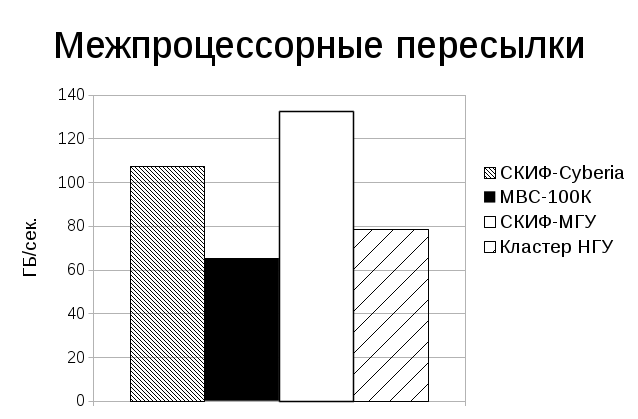
\includegraphics[height=7cm,keepaspectratio]{images/particle_send_GBsec.png}
				\end{center}
				\caption{Скорость пересылки данных на некоторых кластерах. Количество модельных частиц: 2.5 млн. на каждое процессорное ядро. Измерения выполнены в 2010 г.}
				\label{procs_flops}
			\end{figure}
			
			Измеренная таким образом скорость пересылки данных показывает фактический предел этой величины, реально достижимый для вычислительного приложения с использованием имеющегося оборудования и коммуникационного программного обеспечения. Это подтверждается следующими соображениями:
			\begin{itemize}
				\item Объем пересылаемых данных мал: в среднем 6 Мб на процесс
				\item Соседние MPI-процессы, как правило, расположены на близких узлах.
			\end{itemize}  	 
			
		%	\subsubsection{Экстраполяция результатов тестирования ускорения и эффективности распараллеливания}
			%%	формулы из статьи НГУ-ИТ'17, адаптированные и улучшенные, сравнение со Степаненко
			%%	выводы по большой системе на тех же принципах, совпадение с реальностью
			%%	
			%	В \textit{четвертом разделе} описана оригинальная методика экстраполяции результатов на системы большой размерности и ее сравнение с аналогиными работами.Проведено большое количество физических расчетов с использованием программы в трехмерной расчетной области, использующей двухступенчатую эйлерово-лагранжеву декомпозицию расчетной области.На основании тестовых расчетов на небольшом количестве процессорных ядер измереятся время коллективных и парных коммуникаций MPI и строится аппроксимацию времени пересылок для произвольного количества процессов.
			
			%	Основным вопросом является соответствие реально измеряемого времени выполнения коммуникационных операций для определенного количества процессоров, 
			%	 По результатам вырабатываются рекомендации по выбору оптимального сочетания эйлеровой и лагранжевой декомпозиции.
			%	\textbf{формулы}
			
			%	\subsection{Глава 3: Анализ производительности системы памяти}
			%	\subsubsection{Кэш-память}    
			%	Статьи PACO (кэш, списки и пр.), BOE (данны исполения на Sun Sparc Opteron)
			%	\subsubsection{Оперативная память}
			%	 PAVT10, Абрау7 PACO